\documentclass{article}
\usepackage[T1]{fontenc}
\usepackage[utf8]{inputenc}
\usepackage{amsmath}
\usepackage{amssymb}
\usepackage{hyperref}
\usepackage{parskip} %skip the indent of a new paragraph.
\usepackage{float}
\usepackage{graphicx}
\usepackage{listings}
\usepackage{siunitx}
\usepackage[super]{nth}
\lstset{language=Matlab, frame=single, breaklines=true,numbers=left, keywordstyle=\color{blue},rulecolor=\color{black},commentstyle=\color{gray}}

\usepackage{cleveref}
\usepackage{todonotes}

%% Brukes for tabeller (av likninger)
\usepackage{tabularx}
\def\tabularxcolumn#1{m{#1}}

\newcommand{\TODO}[1]{\todo[inline]{#1}}
\newcommand{\mbf}[1]{\mathbf{#1}} % Arg 1 is bold (in math environment)
\newcommand{\partialderiv}[2]{\frac{\partial{#1}}{\partial{#2}}} % prints partial derivative as a fraction

\title{Linear Systems TTK4115 - Boat Lab Report}
\author{Bern Johan Damslora -- 759477 \\ Didrik rokhaug -- 759528}
\date{\today}

\begin{document}

% !TEX root = main.tex

\begin{titlepage}
    %\maketitle
    %\rule{\linewidth}{0.5mm}
    \begin{center}
    	\large
    	Linear Systems TTK4115
    \end{center}
    \vspace{\fill}
    \rule{\linewidth}{0.5mm}
    \begin{center}
    	\huge
    	Boat Lab Report
    \end{center}
	\rule{\linewidth}{0.5mm}
	\vspace{\fill}

	%\begin{center}
    %	\huge
    %	Bern Johan Damslora -- 759477 \\ Didrik rokhaug -- 759528
    %\end{center}
    \large
    \centering
    Group 33:
    \begin{table}[H]
    	\centering
    	\large
    	\begin{tabular}{rl}
    		\textbf{Bernt Johan Damslora} & (nr. 759477) \\
    		\textbf{Didrik Rokhaug} &  (nr. 759528)

    	\end{tabular}
    \end{table}
    \vspace{\fill}
    \begin{center}
    	\large
    	\today
    \end{center}
	\vspace{\fill}
    \begin{figure}[H]
    \centering
    \includegraphics[width=0.5\textwidth]{images/logontnu_eng}
    \end{figure}
    \thispagestyle{empty}
\end{titlepage}


%\section*{Table of contents}
\tableofcontents
\thispagestyle{empty} %Avoid page numbering on the table of contents
\newpage

\setcounter{page}{1}
% Part 1
% !TEX root = main.tex
\section{Part 1: Identification of the boat  parameters}

In the assignment text we were given the following model of a ship:
\begin{subequations}
	\label{eq:completeModel}
		\begin{align}
				\dot{\xi_w} &= \psi_w \label{eq:xi_w}\\
				\dot{\psi_w} &= -\omega_0^2\xi_w-2\lambda\omega_0\psi_w+K_ww_w \label{eq:psi_w}\\
				\dot{\psi} &= r \label{eq:psi} \\
				\dot{r} &= -\frac{1}{T}r+\frac{K}{T}(\delta-b) \label{eq:r} \\
				\dot{b} &= w_b \label{eq:b} \\
				y &= \psi + \psi_w + v \label{eq:y}
		\end{align}
\end{subequations}

Where $\psi$ is the average heading, $\psi_w$ is a high frequency component due to the wave disturbance, $r$ the yaw rate and $b$ is a bias to the rudder angle $\delta$, $w_w$ and $w_b$ are white noice disturbances, $v$ is meassurement noise and $K$, $T$, $\lambda$ and $\omega_0$ are model parameters.


\subsection{1a)}

Using this model we can find the transfer function from $\delta$ to $\psi$. Taking the laplace transform of \cref{eq:psi} and \cref{eq:r} yields
\begin{subequations}
	\begin{align}
		s\psi &= r \label{eq:Lpsi}\\
		sr &= -\frac{1}{T}r + \frac{K}{T}(\delta-b) \label{eq:Lr}
	\end{align}
\end{subequations}

Assuming no disturbances $b = 0$ and combining \cref{eq:Lpsi} with \cref{eq:Lr} gives
\begin{equation}
	H_{ship}(s) = \frac{\psi}{\delta}(s) = \frac{K}{s^2T+s} \label{eq:H(s)}
\end{equation}

\subsection{1b)}

To find $K$ and $T$ we use the frequency response of \cref{eq:H(s)} with the frequencies $\omega_1 = 0.005\si{\radian\per\second}$ and $\omega_2 = 0.05\si{\radian\per\second}$, both with an amplitude of $1$. Using the provided ``ship'' we found the amplitudes experimentally (see \cref{fig:sin0.005} and \cref{fig:sin0.05}). This yields the equations
\begin{subequations}
	\begin{align}
		|H_{ship}(j\omega_1)| &= \frac{K}{\sqrt{T^2\omega_1^4 + \omega_1^2}} = 31.9787 \label{eq:omega_1}\\
		|H_{ship}(j\omega_2)| &= \frac{K}{\sqrt{T^2\omega_2^4 + \omega_2^2}} = 0.7847 \label{eq:omega_2}
	\end{align}
\end{subequations}

\begin{figure}
	\centering
	\includegraphics[width=\textwidth]{images/oppg1/sin0005.pdf}
	\caption{Response of the ship given a input of \ensuremath{\sin{0.005}}.
		Blue line is without any noise, red line is with both waves and meassurement noise.}
	\label{fig:sin0.005}
\end{figure}

\begin{figure}
	\centering
	\includegraphics[width=\textwidth]{images/oppg1/sin005.pdf}
	\caption{Response of the ship given a input of \ensuremath{\sin{0.05}}.
		Blue line is without any noise, red line is with both waves and meassurement noise.}
	\label{fig:sin0.05}
\end{figure}

Using MatLab function \texttt{solve} to solve this set of equations numerically yields
\begin{subequations}
	\begin{align}
		K &= 0.1742 \\
		T &= 86.5246
	\end{align}
\end{subequations}

\subsection{1c)}

If we simulate the ship with disturbance we see from \cref{fig:sin0.005}  and \cref{fig:sin0.05} that we get a noise component on top of the sinusoidal response. This makes it hard to find the true amplitude of the response, as we cannot simply use the half difference between the maximum and minimum.

\subsection{1d)}

If we apply a step input of $1$ degree at $t=0$ we get the response seen in \cref{fig:step_1}. As we can see the model is close to the ``actual'' ship at the beginning, but as the time increases, so does the errors of the model. This means that for small $t$s the model is a good approximation.

\begin{figure}
	\centering
	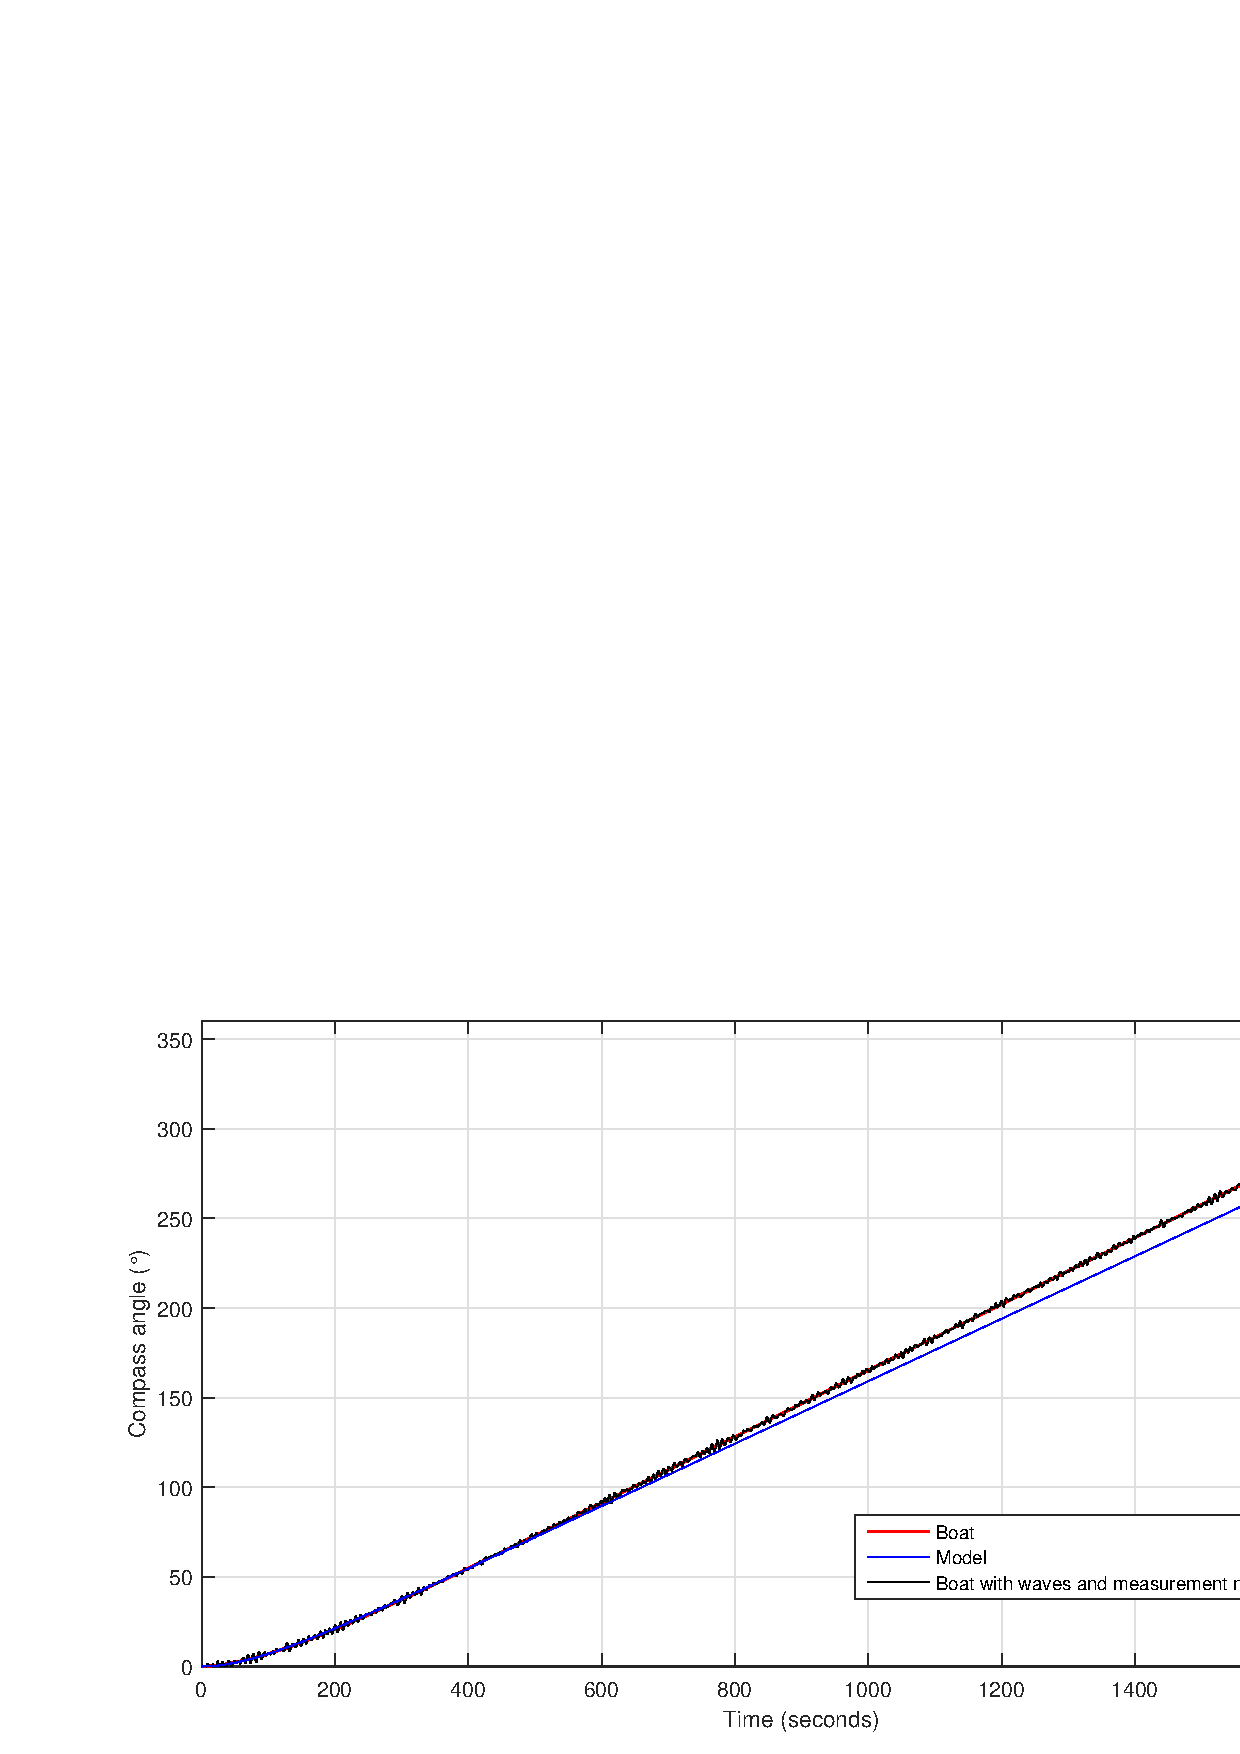
\includegraphics[width=\textwidth]{images/oppg1/step1_with_model_trafu.pdf}
	\caption{Position of the ship and the model given a step input}
	\label{fig:step_1}
\end{figure}


% Part 2
% !TEX root = main.tex

\section{Part 2: Identification of wave spectrum model}

\subsection{2a)}

% Si noe om hva oppgaven er (finne \omega_0 og \lambda)

\todo[inline, author=Didrik]{Vil Bernt Johan skrive dette som har gjort det?}

\subsection{2b)}
To find the values of $\omega_0$ and $\lambda$ we can compare the estimated PSD of the waves with an analytical, found by using the model of the waves. In order to do this we first need to find the transfer function from $w_w$ to $\psi_w$. This can be done by taking the laplace transform of \cref{eq:xi_w} and \cref{eq:psi_w} yielding

\begin{equation}
    G(s) = \frac{\psi_w}{w_w}(s) = K_w\frac{s}{s^2+2\lambda\omega_0s+\omega_0^2} \label{eq:G(s)}
\end{equation}

To find the power spectral density function we use that $S_y(\omega) = |H(j\omega)|^2S_u(\omega)$. This means

\begin{equation}
    P_{\psi_w}(\omega) = |G(j\omega)|^2 = K_w^2\frac{\omega^2}{\omega^4+2\omega_0^2(2\lambda^2-1)\omega^2+\omega_0^4} \label{eq:PSD}
\end{equation}


\subsection{2c)}
\todo[inline]{Skriv stuff her}

\subsection{2d)}
\todo[inline]{Skriv stuff her}


% Part 3
% !TEX root=main.tex

\section{Part 3: Control system design}

\subsection{3a)}

We want to design a limited PD controller with the transfer function

\begin{equation}
    H_{pd}(s) = K_{pd}\frac{1+T_ds}{1+T_fs} \label{eq:H_pd}
\end{equation}

to control the heading $\psi$ of the ship, by setting the rudder angle $\delta$. We want the cross frequency and phase margin of the open loop system to be $0.10\si{\radian\per\second}$ and $50$ degrees respectively. We also want the time constant $T_d$ to equal the time constant of the system. In order to choose $K_{pd}$, $T_d$ and $T_f$ we first find the transfer function of the open loop system

\begin{equation}
    H_{sys}(s) = H_{pd}(s) \cdot H_{ship}(s) = KK_{pd}\frac{1+T_ds}{s(Ts+1)(T_fs+1)} \label{eq:H_sys}
\end{equation}

As we want $T_d$ to equal the time constant of the model we set $T_d = T = 86.5246 \si{\second}$. Next we use that the phase margin of a system is equal to $\angle H(j\omega_c) + 180 \si{\degree}$.

\begin{subequations}
    \begin{align}
        \angle H_{sys}(j\omega_c) + 180 \si{\degree} &= 50 \si{\degree} \\
        \angle \frac{KK_{pd}}{(j\omega_c)^2T_f+j\omega_c} &= -130 \si{\degree}\\
        \angle KK_{pd} - \angle ((j\omega_c)^2T_f+j\omega_c) &= -130 \si{\degree} \\
        \angle ((j\omega_c)^2T_f+j\omega_c) &= -130\si{\degree} \\
        \tan^{-1}\frac{\omega_c}{\omega_c^2T_f} &= 50 \si{\degree} \\
        T_f &= \frac{1}{ \omega_c \tan (50 \si{\degree}) } \\
        T_f &= 8.3910 \si{\second} \label{eq:T_f}
    \end{align}
\end{subequations}

Last we find $K_{pd}$ by using the definition of the cross frequency: $|H(j\omega_c)| = 1$. This yields

\begin{subequations}
    \begin{align}
        |H_{sys}(j\omega_c) &= 1 \\
        |H_{sys}^2(j\omega_c) &= 1^2 \\
        \left | \frac{KK_{pd}}{s^2T_f+s} \right |^2 &= 1 \\
        \frac{(KK_{pd})^2}{(\omega_c^2 T_f)^2 + \omega_c^2} &= 1 \\
        K_{pd} &= \frac{\sqrt{(\omega_c^2 T_f)^2} + \omega_c^2}{K} \label{eq:K_pd(T_f)}
    \end{align}
\end{subequations}

Inserting \cref{eq:T_f} into \cref{eq:K_pd(T_f)} yields a $K_{pd} = 0.7494$. The controller was implemented in Simulink as seen in \cref{fig:pd}.

\begin{figure}
    \centering
    \includegraphics[width=\textwidth]{images/oppg3/a_pd-loop.pdf}
    \caption{Simulink implementation of the PD-controller}
    \label{fig:pd}
\end{figure}

\subsection{3b)}

As we can see in \cref{fig:step_no_dist} the controller does a good job when there are no disturbances. The ship reaches the reference $\psi_r$ of $30\si{\degree}$ within 2 minutes, and the rudder angle is relatively constant over time.

\begin{figure}
    \centering
    \includegraphics[width=\textwidth]{images/oppg3/stepresp_no_disturbance.eps}
    \caption{Step response of the controller. No disturances.}
    \label{fig:step_no_dist}
\end{figure}

\subsection{3c)}

In \cref{fig:step_current_dist} we see the response of the controller with current disturbance. as we can see the controller is unable to counteract the constant disturbance of the current, which leads to a large constant deviation from the setpoint.

\begin{figure}
    \centering
    \includegraphics[width=\textwidth]{images/oppg3/stepresp_current_disturbance.eps}
    \caption{Step response of the controller. With current disturbance.}
    \label{fig:step_current_dist}
\end{figure}

\subsection{3d)}

When we apply wave current (and turn off current disturbance), we see that the controller does it best to remove the noise but is unable to do much. In its attempt to remove the noise it applies a lot of rudder input, which if the boat was real would stress the physical system.

\begin{figure}
    \centering
    \includegraphics[width=\textwidth]{images/oppg3/stepresp_wave_disturbance.eps}
    \caption{Step response of the controller. With wave disturbance}
    \label{fig:step_wave_dist}
\end{figure}


% Osv.

%uncomment to add reference list
%\newpage
%\input{reference}

\end{document}
